 
\chapter{Ordinary Least Squares with a Univariate Covariate}
 \label{chapter::ols-1d}
 
 
This chapter discusses ordinary least squares (OLS) with a single covariate. It can provide insights into later chapters because it is the building block of OLS with multiple covariates.
 

\section{Ordinary least squares with a univariate covariate}
Figure \ref{fig::galton_data_scatterplot} shows the scatterplot of Galton's dataset which can be found in the \ri{R} package \ri{HistData} as \ri{GaltonFamilies}. In this dataset, \ri{father} denotes the height of the father and \ri{mother} denotes the height of the mother. 
 The x-axis denotes the mid-parent height, calculated as (\ri{father} + 1.08*\ri{mother})/2, and the y-axis denotes the height of a child. 



\begin{figure}[ht]
\centering
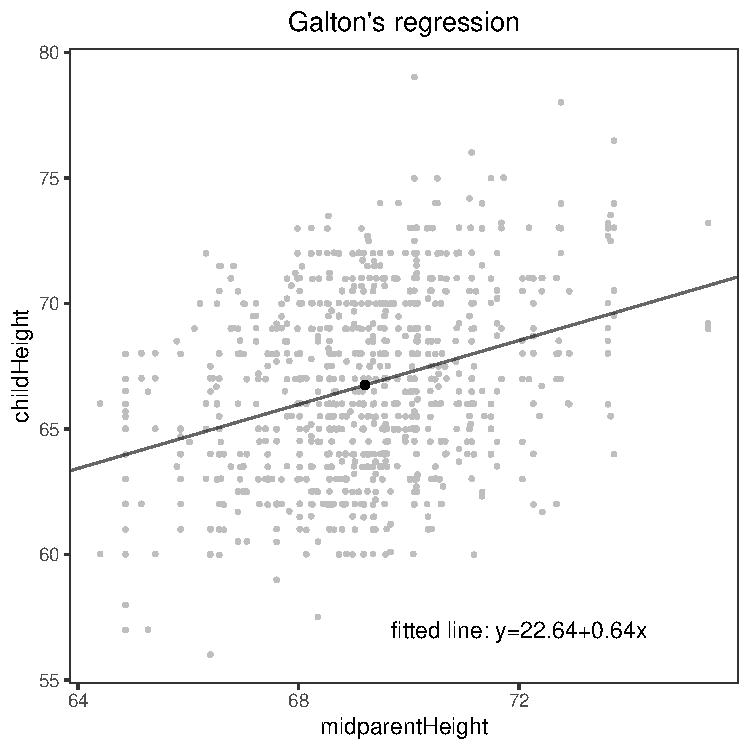
\includegraphics[width= 0.7\textwidth]{figures/galton_data_ggplot.pdf}
\caption{Galton's dataset}\label{fig::galton_data_scatterplot}
\end{figure}


With $n$ data points $(x_{i,}y_{i})_{i=1}^{n}$, our goal is to find the best linear fit of the data
\[
(x_{i,}\hat{y}_{i}=\hat{\alpha}+\hat{\beta}x_{i})_{i=1}^{n},
\]
where the coefficients $\hat{\alpha}$ and $\hat{\beta}$ are determined from the data. 
What do we mean by the ``best'' fit? Gauss proposed to use the following OLS criterion:\footnote{The idea of OLS is often attributed to Gauss and Legendre. Gauss used it in the process of discovering Ceres, and his work was published in 1809. Legendre's work appeared in 1805 but Gauss claimed that he had been using it since 1794 or 1795. \citet{stigler1981gauss} reviews the history of OLS.}
\begin{equation}
\label{eq::ols-univariate-objective}
(\hat{\alpha},\hat{\beta})=\arg\min_{a,b}n^{-1}\sumn(y_{i}-a-b x_{i})^{2}.
\end{equation}

The OLS criterion is based on the squared ``misfits'' $y_{i}- a - b  x_{i}$. Another intuitive criterion is based on the absolute values of those misfits, which is called the least absolute deviation (LAD). However, OLS is simpler because the objective function is smooth in $(a, b)$, and we can obtain close-form solutions. I will discuss LAD in Chapter \ref{chapter::quantile-regression} as a special case of {\it quantile regression}. 


How do we solve the OLS minimization problem in \eqref{eq::ols-univariate-objective}? The objective function
is quadratic, and as $a$ and $b$ diverge, it diverges to
infinity. So it must have a minimizer $(\hat{\alpha},\hat{\beta})$, which satisfies the first-order condition:
\begin{eqnarray}
-\frac{2}{n}\sumn(y_{i}-\hat{\alpha}-\hat{\beta}x_{i}) & = &0,\label{eq::univariate-foc-1} \\
-\frac{2}{n}\sumn x_{i}(y_{i}-\hat{\alpha}-\hat{\beta}x_{i}) & =&0.\label{eq::univariate-foc-2}
\end{eqnarray}
The equations \eqref{eq::univariate-foc-1} and \eqref{eq::univariate-foc-2} are called the Normal Equations of OLS. The first
equation \eqref{eq::univariate-foc-1} implies 
\begin{equation}
\bar{y}=\hat{\alpha}+\hat{\beta}\bar{x},\label{eq:normal1}
\end{equation}
that is, the OLS line must go through the sample mean of the data $(\bar{x},\bar{y}).$ The second equation \eqref{eq::univariate-foc-2} implies
\begin{equation}
\overline{xy}=\hat{\alpha}\bar{x}+\hat{\beta}\overline{x^{2},}\label{eq:normal2}
\end{equation}
where $\overline{xy}$ is the sample mean of the $x_{i}y_{i}$'s, and $\overline{x^{2}}$
is the sample mean of the $x_{i}^{2}$'s. Subtracting (\ref{eq:normal1})$\times\bar{x}$
from (\ref{eq:normal2}), we have
$$
\overline{xy} - \bar{x} \bar{y} = \hat{\beta} ( \overline{x^{2}} - \bar{x}^2 ) ,
$$
which is
$$
\hat{\sigma}_{xy} =\hat{\beta} \hat{\sigma}_{x}^2 ,
$$
and implies
\begin{equation}
\label{eq::ols-slope}
\hat{\beta} =   \frac{\hat{\sigma}_{xy}}{\hat{\sigma}_{x}^2}. 
\end{equation}
So the OLS coefficient of $x$ equals the sample covariance between
$x$ and $y$ divided by the sample variance of $x$. From (\ref{eq:normal1}),
we obtain that 
\begin{equation}
\label{eq::ols-intercept}
\hat{\alpha}=\bar{y}-\hat{\beta}\bar{x}.
\end{equation}
By \eqref{eq::ols-intercept}, the fitted line $\hat{y}_i  =\hat{\alpha}+\hat{\beta}x_i$ simplifies to $\hat{y}_i  = \bar{y}-\hat{\beta}\bar{x}+\hat{\beta}x_i$, and more symmetrically, $\hat{y}_i -\bar{y}=\hat{\beta}(x_i-\bar{x})$. With \eqref{eq::ols-slope}, we can further simplify the fitted line as
\begin{eqnarray*}
\hat{y}_i -\bar{y} &=& \frac{   \hat{\sigma}_{xy}  }{  \hat{\sigma}_{x}^2  }(x_i-\bar{x}) \\
 &=&\frac{  \hat{\rho}_{xy} \hat{\sigma}_{x}\hat{\sigma}_{y}}{\hat{\sigma}_{x}^{2}}(x_i-\bar{x}),
\end{eqnarray*}
which implies
$$
\frac{\hat{y}_i -\bar{y}}{\hat{\sigma}_{y}}= \hat{\rho}_{xy}  \frac{x_i-\bar{x}}{\hat{\sigma}_{x}},
$$
the Galtonian formula mentioned in Chapter \ref{chapter::motivation}. 



%Why statistics? The above OLS results are purely algebraic, that is,
%finding the best linear fit to $n$ points. If this is the only goal,
%then we do not need to impose any additional assumptions in the above
%procedure. However, we want to make inference based on OLS. Here inference
%means quantifying uncertainty. But before quantifying uncertainty,
%we need to explicitly state the truth we want to infer. 
%
%
%One possible
%model is that $(x_{i},y_{i})_{i=1}^{n}$ are IID and
%\[
%y_{i}=\alpha+\beta x_{i}+\varepsilon_{i}\qquad(i=1,\ldots,n)
%\]
%where the outcome variable $y_{i}$ on the left-hand side is generated
%based on $x_{i}$ and $\varepsilon_{i}$ on the right-hand side. We
%can view the $\varepsilon_{i}$ term as random errors that satisfies
%\[
%\begin{cases}
%E(\varepsilon_{i}) & =0,\\
%E(\varepsilon_{i}x_{i}) & =0.
%\end{cases}
%\]
%
%Under this model, $(x_{i},y_{i})_{i=1}^{n}$ are random, so are $\hat{\alpha}$
%and $\hat{\beta}$. Then we can discuss the distributional properties
%of $\hat{\alpha}$ and $\hat{\beta}$, for example, their means, variances,
%and sampling distributions. 
%\section{Galton's data}


We can obtain the fitted line based on Galton's data using the \ri{R} code below. 

\begin{rc}
> library("HistData")
> xx = GaltonFamilies$midparentHeight
> yy = GaltonFamilies$childHeight
> 
> center_x = mean(xx)
> center_y = mean(yy)
> sd_x     = sd(xx)
> sd_y     = sd(yy)
> rho_xy   = cor(xx, yy)
> 
> beta_fit  = rho_xy*sd_y/sd_x
> alpha_fit = center_y - beta_fit*center_x
> alpha_fit
[1] 22.63624
> beta_fit
[1] 0.6373609
\end{rc}

I then generate Figure \ref{fig::galton_data_scatterplot} based on the original data and the OLS coefficients. 




\section{Final comments}\label{section::1d-comments}

I make two final comments on OLS. 
\begin{enumerate}[label=(C\arabic*), ref=C\arabic*]
\item
We can write the sample mean as the solution to the OLS with only the intercept:
\begin{equation}\label{eq::ols-mean}
\bar{y} = \arg\min_{\mu}n^{-1}\sumn(y_{i} - \mu)^{2}.
\end{equation}


\item
We can fit OLS of $y_i$ on $x_i$ without the intercept: 
\[
 \hat{\beta}=\arg\min_{b}n^{-1}\sumn(y_{i} -b x_{i})^{2} 
\]
which equals 
\begin{equation}
\label{eq::ols-without-intercept}
 \hat{\beta} 
 = \frac{ \sumn x_iy_i }{  \sumn x_i^2 } = \frac{  \langle x, y \rangle   }{ \langle x, x \rangle } , 
\end{equation}
 where $x = (x_1, \ldots, x_n)^{\T}$ and $y = (y_1, \ldots, y_n)^{\T}$ are the $n$-dimensional vectors containing all observations, and $\langle x, y \rangle = \sumn x_iy_i$ denotes the inner product between $x$ and $y$. 
 \end{enumerate}
 
 
Although it is rare to fit the above OLS in practical data analysis, the formulas in \eqref{eq::ols-mean} and \eqref{eq::ols-without-intercept} will be the building blocks for many discussions in later parts of the book. I leave the proof of \eqref{eq::ols-mean} and \eqref{eq::ols-without-intercept} as Problem \ref{hw2::univariate-ols-2}. 




\section{Homework problems}

\paragraph{Univariate OLS}\label{hw2::univariate-ols-2}

Prove   \eqref{eq::ols-mean} and \eqref{eq::ols-without-intercept}. 

\paragraph{Pairwise slopes}\label{hw2::pairwise-slope}



Prove Theorem \ref{thm::ols-pairwise-formula} below. 

\begin{theorem}
\label{thm::ols-pairwise-formula}
Given $(x_i, y_i)_{i=1}^n$ with univariate $x_i$ and $y_i$, show that $\hat\beta$ in \eqref{eq::ols-slope} equals
$$
\hat{\beta} = \sum_{(i,j)} w_{ij} b_{ij},
$$
where the summation is over all pairs of observations $(i,j)$, 
$$
b_{ij} = \frac{ y_i - y_j }{  x_i - x_j } 
$$
is the slope determined by two points $(x_i,y_i)$ and $(x_j, y_j)$, and 
$$
w_{ij} = \frac{  x_i - x_j)^2 }{   \sum_{(i',j')} (x_{i'} - x_{j'})^2 } 
$$
is the weight proportional to the squared distance between $x_i$ and $x_j$. In the above formulas, if $x_i=x_j$, then we define $b_{ij} = 0$, and the corresponding weight $w_{ij}$ equals $0$. 
\end{theorem}

 

Remark: \citet{wu1986jackknife} and \citet{gelman2009splitting} used Theorem \ref{thm::ols-pairwise-formula}. 
Problem \ref{hw03::jacobi} gives a more general result. 


 
\paragraph{No regression}\label{hw2::no-regression}

\begin{figure}
\centering
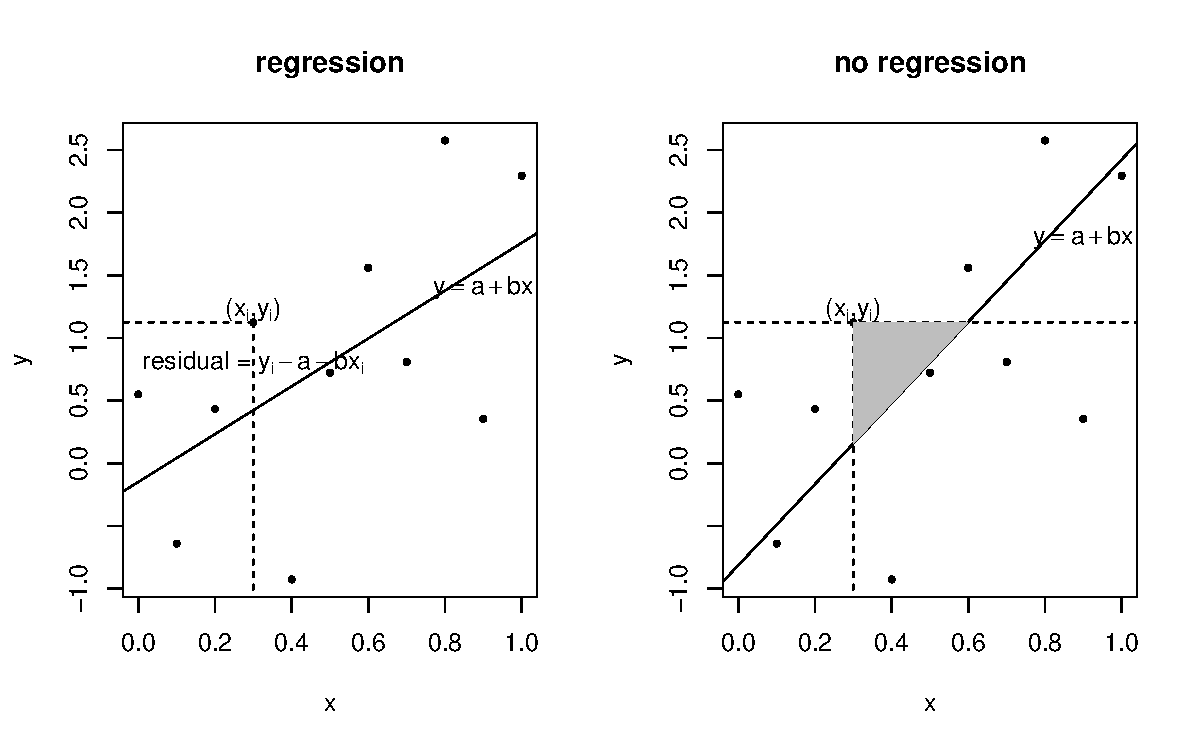
\includegraphics[width =\textwidth]{figures/regression_no_regression.pdf}
\caption{Regression (left) and no regression (right)}
\label{fig::no-regression}
\end{figure}


\citet{woolley1941method} proposed a method to minimize the sum of the areas formed between the data points and fitted line. The right panel of Figure \ref{fig::no-regression} illustrates the area formed between data point $(x_i, y_i)$ and the line $y=a+bx$. 

Prove that if $\hat{\rho}_{xy}>0$, then the minimizer $(\hat\alpha', \hat\beta')$ satisfies
$$
\hat\beta '  = \frac{\hat\sigma_y}{\hat\sigma_x}
$$
and
$$
\hat\alpha '  = \bar{y} - \hat\beta  \bar{x}.
$$

Remark: The fitted line is
\begin{eqnarray*}
\hat{y}_i 
&=& \hat\alpha '  + \hat\beta '  x_i  \\
&=& \bar{y} - \hat\beta  \bar{x} + \hat\beta '  x_i , 
\end{eqnarray*}
which is equivalent to
$$
\frac{\hat{y}_i-\bar{y}}{\hat{\sigma}_{y}}=   \frac{x_i-\bar{x}}{\hat{\sigma}_{x}} .
$$
It does not have the regression factor $\hat{\rho}_{xy}$, compared with the Galtonian formula, which is derived by minimizing the residual sum of squares as illustrated by the left panel of Figure \ref{fig::no-regression}. 
 



 
 
 
